\SubCity{Eldaarich}
{21,000 (85\% humans, 8\% dwarves, 4\% half-giants, 2\% muls, 1\% others).}
{Gold, silver.}
{Eldaarish, picts.}
{
\begin{figure*}[b!]
\centering
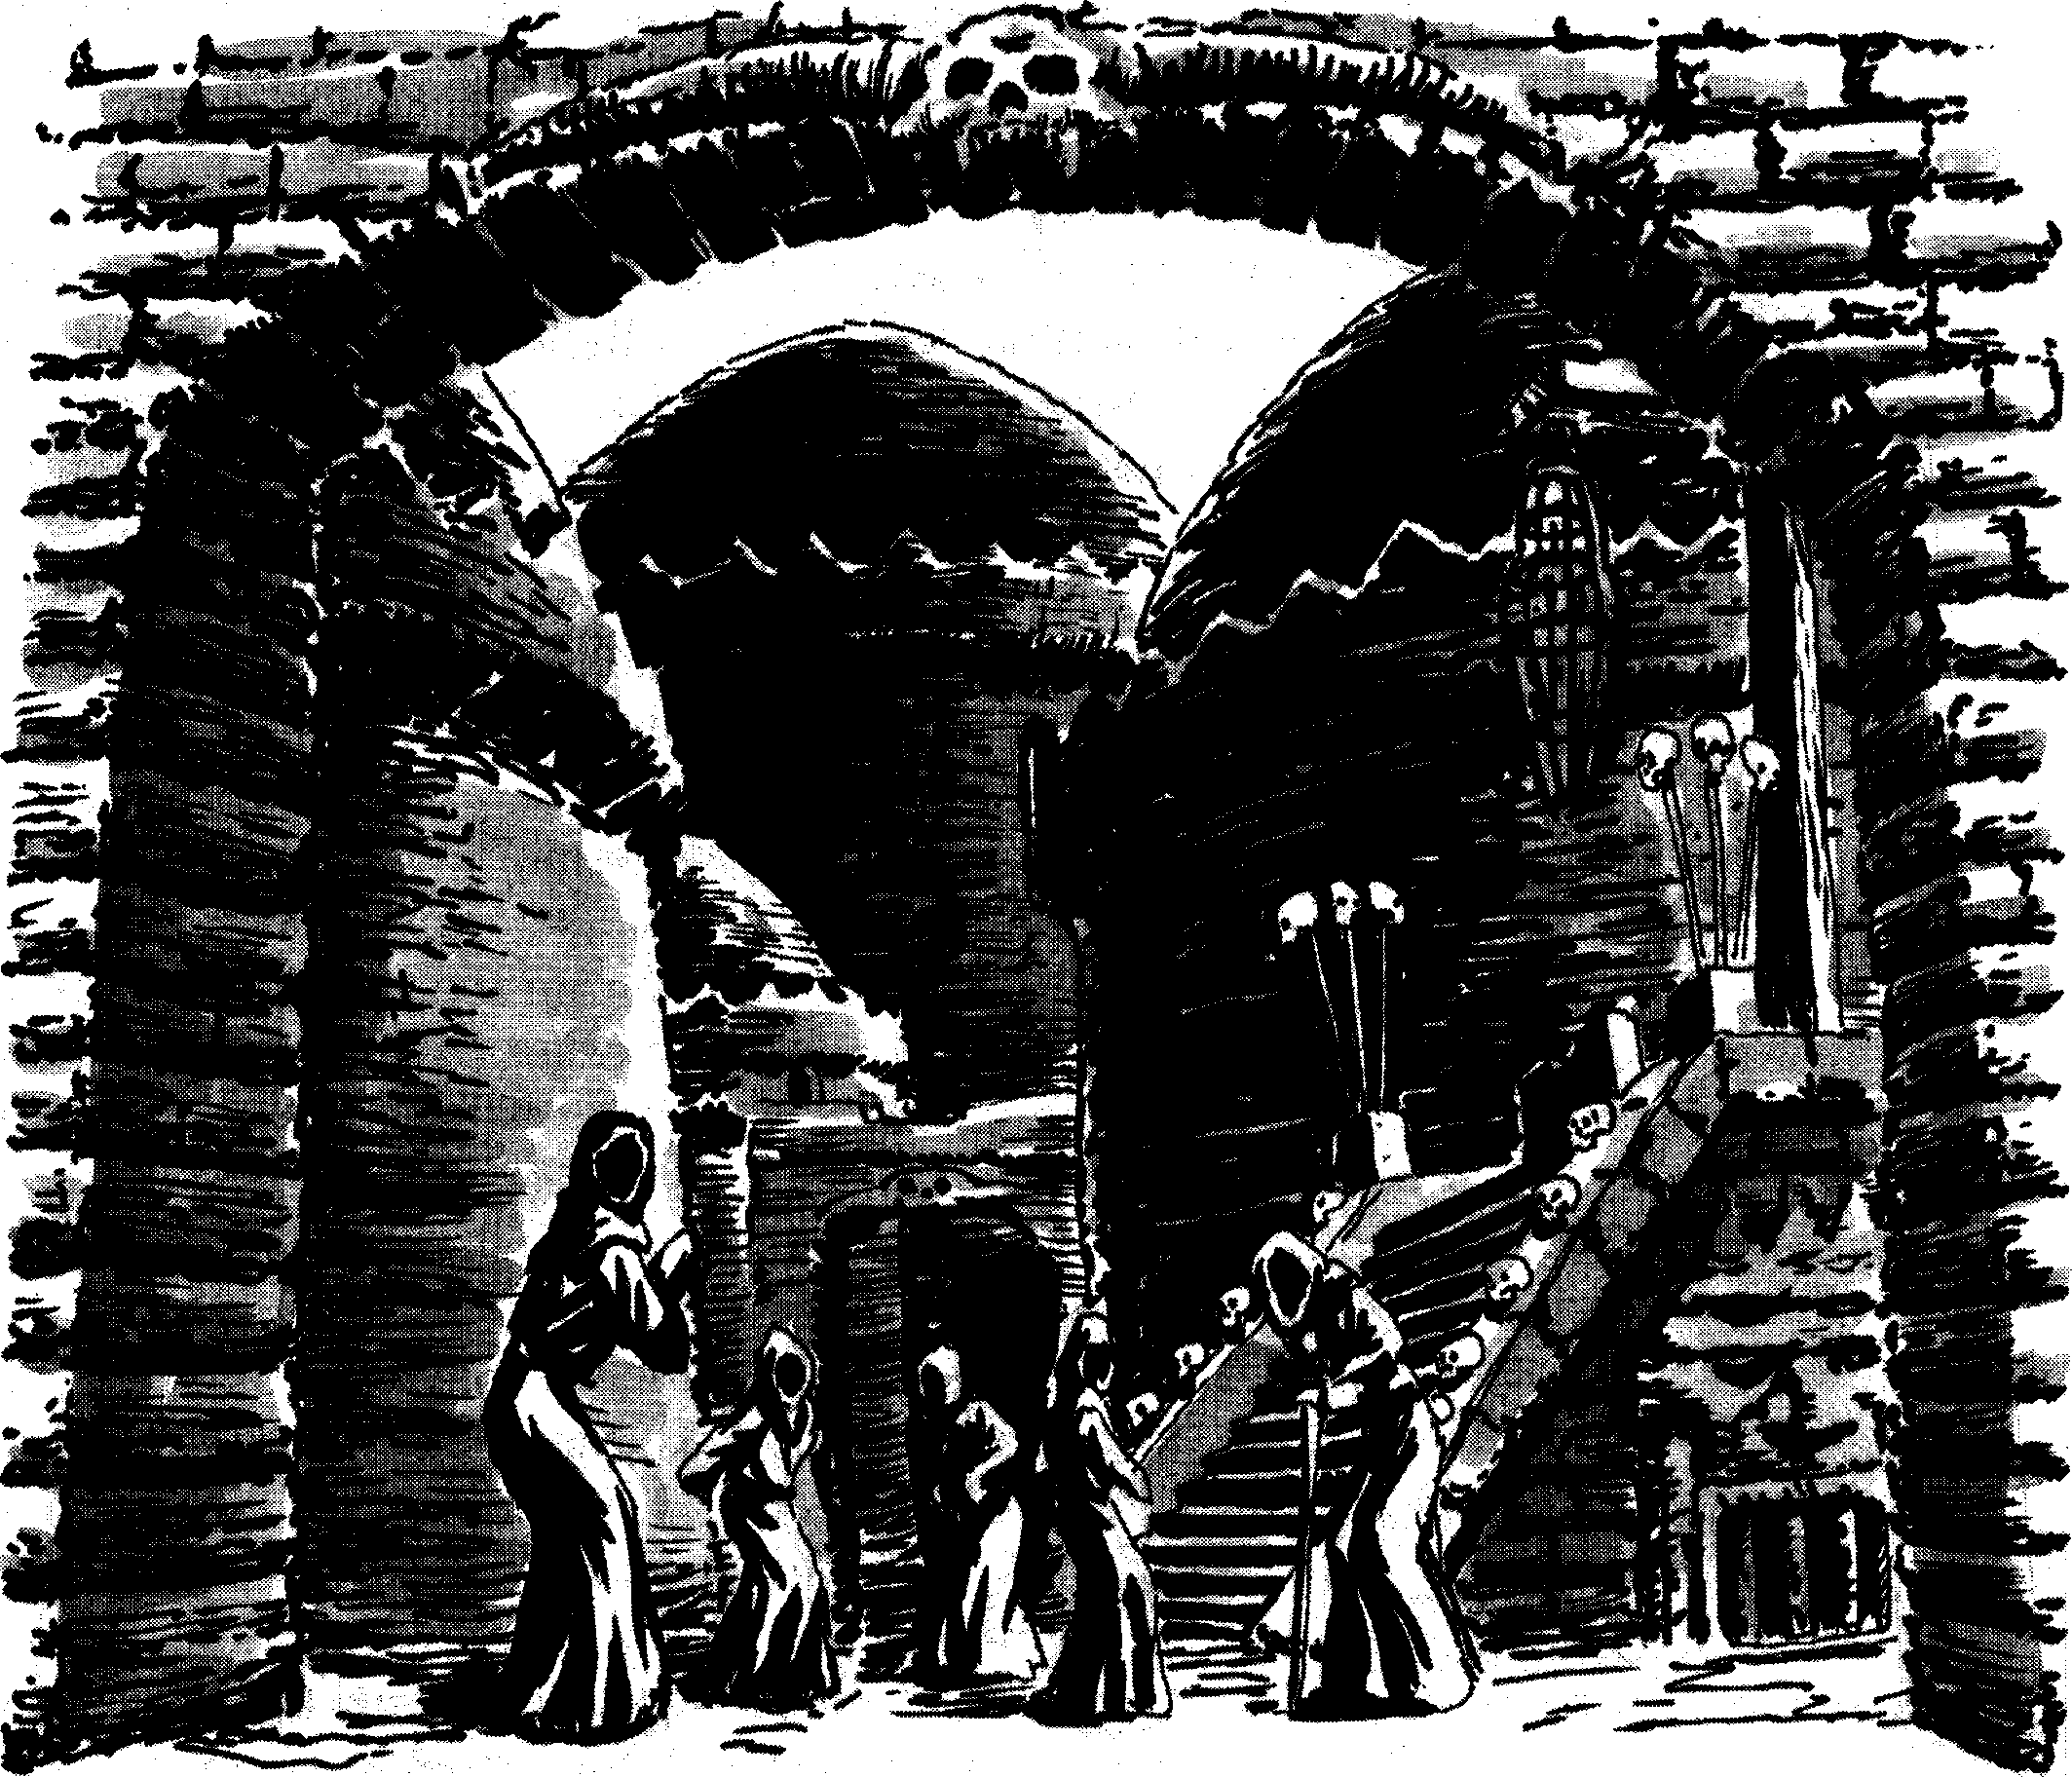
\includegraphics[height=0.4\paperheight]{images/eldaarich-1.png}
\par\textit{\small\textcopyright Wizards of the Coast, 2020.}
\end{figure*}

	Eldaarich occupies a small island in the Sea of Silt, just off the mainland. Here, isolated and protected from the rest of Athas, the citizens huddle in the paranoid delusions of their mad sorcerer-king. Daskinor, ruler of Eldaarich, believes that unknowable forces in the world are trying to destroy him.

	Every few years he puts a new name to these forces---the Order, the Veiled Alliance, Rajaat, pyreen, a merchant house, a lowly slave, or some other identifiable target becomes the imagined source of his fears for a time. Daskinor does his best to destroy these imagined enemies, and anyone who has even a passing resemblance to the target is persecuted until the next delusion grips him.

	Daskinor was never a stable ruler. From the beginning of his reign as sorcerer-king of Eldaarich, he was tormented by unfounded fears and nameless terrors that preyed upon his mind. For the first few centuries of his reign, he was able to function more or less normally despite his growing paranoia. As time passed, genuine bouts of panic began to intrude upon his psyche. These bouts lasted longer and longer, paralyzing Daskinor for hours, days, sometimes even months at a time.

	Eldaarich was constructed to protect Daskinor from his fears. Fortified walls, a strong military, devoted templars, retractable bridges, and a series of keeps and forts ensured that the entire city-state and surrounding area was secured against outsiders. Over time, it became less of a fort and more of a prison, locking king and citizens alike behind sturdy gates and high walls. Seven centuries ago, the sorcerer-king's paranoia became acute. He completely sealed his city, cutting off all ties to the other city-states. That was the way things remained until about FY 0 year, when limited trade was resumed with House Azeth of Kurn.

	Today, Eldaarich remains an isolated prison of a city. Daskinor's fears have become the fears of his citizenry, making everyone who lives under his rule as paranoid as he is. No one ever leaves Eldaarich, and no one ever enters its massive gates. It's a closed society---figuratively and literally.
}
{
	Every outsider wants to destroy their city-state and their sorcerer-king, and everyone who lives within the walls waits for an opportunity to betray you. That's what the people of Eldaarich believe, for that's what their leaders believe. Nowhere else in all of Athas is there such an underlying current of genuine, unattributable fear. It filters down from Daskinor himself, making citizen and slave alike tremble with uncontrollable paranoia.

	The citizenry is a subdued, cowering lot, given to unexpected bursts of violence once the fear inside them becomes too much to contain. In many cases, the ever-crushing weight of terror and oppression keeps the masses down, but sometimes a delusional artisan will strike out at a templar or noble, causing the level of paranoia to rise even higher.

	The quality of life isn't good in Eldaarich. Because Daskinor doesn't trust anyone, he allows his templars to dispense only the barest essentials to the free citizens and slaves. With just enough food and water to sustain them and few personal possessions, the people of the city are a sad, pathetic lot. They have no hope of a better life and no concept that a better life exists outside the walls of Eldaarich. If anyone even suggests such a notion, the ingrained fear of the unknown kicks in and makes everyone else dismiss the idea.

	While the class structure of noble, free citizen and slave exists in Eldaarich, the truth is that everyone beneath the templars is a slave to Daskinor's all-pervasive fear.

	The sorcerer-king sees threats to his rule on every face and in every dark shadow. For this reason, he permits no freedoms of any sort, not even the token rights given to the citizens of other cities. Freedom, Daskinor believes, is just an opportunity to betray his trust. So he orders his templars to oppress the people of his city, to make their lives so miserable they don't have time or strength to contemplate treachery.

	The templars don't have it much better. They're kept in line by the high templars who, in turn, are subject to Daskinor's brutal whims.

	The majority of the population consists of humans, though there are also dwarves, half-giants, and muls in significant numbers. There are also a few aarakocra wasting away in the slave pens. Daskinor has a particular hatred of the winged people and gives his templars special compensations for capturing aarakocra from the nearby White Mountains.

	If travelers were to find themselves in Eldaarich or one of its holdings (which isn't very likely), they'd feel the weight of oppression and smell the stench of mental illness that hangs in the hot, stifling air. Every year the darkness in Daskinor's soul grows deeper, his paranoia more acute. This mental deterioration is reflected in the city itself, as though each citizen were a part of the sorcerer-king's diseased mind.
}
{
	The same model of government evident in the other city-states exists in Eldaarich. The sorcerer-king Daskinor (CE male stage II Champion of Rajaat dragon defiler 8/nomad 10/cerebremancer 10/Athasian dragon 2) stands atop the societal hierarchy, his troubled delusions coloring every aspect of life in the city-state. His chaotic tendencies and often overwhelming paranoia infuse everyone he comes in contact with, making the city almost as wild and frenzied as Raam. The only thing that allows the city to function is that the citizens are a subdued lot, living in quiet fear instead of in rambunctious anarchy. Daskinor constantly watches over his shoulder for assassins that don't exist, and so do his templars and nobles. No one trusts anyone else in Eldaarich. This works out for the best, as the troubled atmosphere has fostered a society where the fear of murder and betrayal has encouraged the periodic use of such techniques by those who prefer to strike first.

	Templars and nobles regularly kill each other to keep the same from happening to them, or to gain power or position, or just because the tension of living behind heavy locks and being constantly on guard eventually drives even the most peaceful beings to violence. In Eldaarich, fears permeates everything---fear of the sorcerer-king, fear of outsiders, fear of each other, and fear of the unknown. Because the society is closed off to the rest of the world, everything on the other side of its walls and locked gates is, by definition, unknown.

	If Eldaarich is a prison, Daskinor is its most prominent prisoner. The sorcerer-king lives in a walled sub-city and rarely ventures into other parts of his realm. His constant paranoia sometimes intensifies to such a fevered pitch that he ceases to function.

	In such a state, which may last as long as months at a time, Daskinor is cared for by his senior templars. At other times, his paranoia drives him to give a name to his fear. When this occurs, the entire city mobilizes to combat this supposed threat to the realm. Currently, the use of psionic abilities has been outlawed, as Daskinor believes that the Order has initiated a campaign against his rule. Even low-powered psionicists and wild talents who openly display their abilities are subject to imprisonment or death because of the current edict. Only Daskinor, a psionicist of the highest caliber, is exempt from the terms of the edict.

	Daskinor's templars serve as administrators to the city, and also act as the sorcerer-king's eyes and ears in all corners of the domain. They are charged with watching for signs of treachery among the masses-and with dealing with such treachery before it gets out of hand. The templars are as paranoid and delusional as Daskinor, giving in to their fear whenever it overwhelms them. For this reason, Eldaarich has become a police state, and the templars are the police. They command the military. They oversee all records and the distribution of goods and services. They hold the power of life and death for the rest of the citizenry in their terrified hands.
}
{
	\textbf{Kulag}: The Kulag Order controls Daskinor's silt fleet, which currently acts as the merchant house for the Dim Lands, a nearby archipelago. It is leaded by High Templar Kerillis (LE female human, templar 14). Sometimes they also resort to piracy in the nearby islands.

	\textbf{Neshtap}: More commonly known as ``red guards'', the Neshtap are the most feared, and the second-most powerful of seven orders that Daskinor uses to maintain control of his city Eldaarich, and its client villages. They never speak, seemingly revere the element of fire, and are becoming increasingly powerful and independent from Daskinor.

	\textbf{The Veiled Alliance}: Eldaarich has no Veiled Alliance. Daskinor rooted out the Alliance and destroyed it 400 years ago when the group of preservers became his imagined enemy of the moment. Some preservers still live in the city, but they remain hidden and are relatively weak due to a lack of adequate training. Preservers from Kurn sometimes sneak into the closed city to provide training and to see what the conditions are, but they don't do this very often. If they get caught, they're put to death, and if their city of origin is discovered, it could mean war between the two cities. No one, especially Oronis the Avangion of Kurn, wants a war to break out. He does, however, feel the pain that both Daskinor and his citizens project, and often contemplates finding a solution to Eldaarich's problems.
}
{}{}
{
	\item A silt schooner owned by House M'ke was attacked and captured by the navy of Eldaarich. The merchant house could hire the PCs to raid the harbor of Eldaarich and bring the schooner back.
	\item An aarakocra from Winter Nest was captured when she flew too close to Eldaarich. The PCs are asked to free her before she is executed by the templars of Eldaarich. Once freed from her cage, the aarakocra can easily fly back to Winter Nest on her own, but the PCs will have to sneak out of Eldaarich.
	\item Grehgatha is a Kurnan preserver who has snuck into Eldaarich many times to tutor young preservers. Since she has returned from her last attempt she is consumed with freeing an entire village from Daskinor and hires the PCs to help. The PCs must come up with a way to sneak 150 people past the templars of Eldaarich.
	\item The Red Guard has become jealous of the monopoly on trade held by the templars of the Kulag Order. In an attempt to disrupt the trade negotiations, the Red Guard mounts a surprise attack on Silt Side during a meeting between Corik Azeth and High Templar Kerillis. The PCs acting as guards for House Azeth may misinterpret the attack as directed by Corik or themselves.
	\item Concerned with a recent rise in the level of the silt sea around Eldaarich, the city has declared war on all silt clerics. Mercenaries are to be hired to help hunt down the silt clerics along the coast for a hundred miles north and south of Eldaarich. The PCs could become embroiled on either side.
	\item A major giant raid on the Huuros Islands has been repulsed by the Kulag Fleet, though many casualties were suffered. Templars assign the PCs to salvage what they can from the battle, equipment as well as the bodies of those who died. Most of the wreckage is just off shore in silt 4.5 to 6 meters deep.
}